% Files using this must be two subfolders
% deep. Adjust the number of ../ for the
% depth of the file.
\providecommand\pointsize{10pt}

\documentclass[\pointsize, letterpaper]{article}

% Imports
\usepackage{fancyhdr}
\usepackage{pgfplots}
\usepackage{geometry}
\usepackage{icomma}
\usepackage{amsmath}
\usepackage{multicol}
\usepackage{mathptmx}
\usepackage{anyfontsize}
\usepackage{t1enc}
\usepackage{tabto}
\usepackage{listings}
\usepackage{filecontents}
\usepackage{subcaption}
\usepackage{tikz}
\usepackage[parfill]{parskip}
\usepackage{graphicx}
\usepackage[]{mdframed}
\usepackage{amsmath}
\usepackage[makeroom]{cancel}
\pgfplotsset{compat=1.18}

\geometry{margin=2.5cm}

\newcommand{\name}{Kaleb Burris}
\newcommand{\classname}{MATH F252, Dr. J. Gimbel}
\newcommand{\assignment}{FILL IN ASSIGNMENT NAME}

\pagestyle{fancy}

\fancyhead[L]{
    \name 
    \newline
    \classname
    \newline
    \assignment
}

\newcommand{\horizontal}{\noindent\rule{\hsize}{0.4pt}}

\setlength{\headheight}{42pt}
\setlength{\headsep}{0.25in}
\setlength{\columnsep}{0.35cm}
\setlength{\columnseprule}{1pt}

% Put the assignment name with \S if 
% necessary for the section and the question 
% numbers.
\renewcommand\assignment{Worksheet 3, due Monday January 25, 4:15pm}

\def\firstcircle{(90:1.75cm) circle (2.5cm)}
\def\secondcircle{(210:1.75cm) circle (2.5cm)}
\def\thirdcircle{(330:1.75cm) circle (2.5cm)}

\begin{document}
    \paragraph*{1.}
    Shade the following events on the Venn diagrams below.
    \begin{multicols}{3}
        \paragraph*{(a)}
        $A \cap (B \cup C)$
        \begin{mdframed}
            \resizebox{\hsize}{!}{\begin{tikzpicture}
                \begin{scope}
                    \clip \firstcircle;
                    \fill[cyan] \thirdcircle;
                    \fill[cyan] \secondcircle;
                \end{scope}
                \draw \firstcircle node[text=black,above] {$A$};
                \draw \secondcircle node [text=black,below left] {$B$};
                \draw \thirdcircle node [text=black,below right] {$C$};
            \end{tikzpicture}}
        \end{mdframed}

        \columnbreak

        \paragraph*{(b)}
        $B \cap A^C$

        \begin{mdframed}

            \resizebox{\hsize}{!}{\begin{tikzpicture}
                \begin{scope}
                    \clip \firstcircle;
                    \clip \thirdcircle;
                    \fill[cyan] \secondcircle;
                \end{scope}
                \draw \firstcircle node[text=black,above] {$A$};
                \draw \secondcircle node [text=black,below left] {$B$};
                \draw \thirdcircle node [text=black,below right] {$C$};
            \end{tikzpicture}}
        \end{mdframed}

        \columnbreak

        \paragraph*{(c)}
        $B \cup (A \cap C)$

        \begin{mdframed}
            \resizebox{\hsize}{!}{\begin{tikzpicture}
                \begin{scope}
                    \clip \secondcircle;
                    \fill[cyan] \firstcircle;
                    \fill[cyan] \thirdcircle;
                \end{scope}
                \draw \firstcircle node[text=black,above] {$A$};
                \draw \secondcircle node [text=black,below left] {$B$};
                \draw \thirdcircle node [text=black,below right] {$C$};
            \end{tikzpicture}}
        \end{mdframed}
    \end{multicols}

    \paragraph*{2.}
    A local Cormac McCarthy club has just voted by secret ballot for the next novel the club members will read. The ballot box contains three slips with votes for book A (“The Road”) and two slips for book B (“No Country For Old Men”). The slips are removed from the box one by one.

    \paragraph*{(a)}
    List all possible outcomes. How many outcomes are there? (For example, one outcome is AABAB.)

    \begin{mdframed}
        \begin{equation*}
            \text{10 Possible outcomes: }
            \left\{
                \begin{array}{l}
                    \{A \quad A \quad A \quad B \quad B\},  \\
                    \{A \quad A \quad B \quad A \quad B\},  \\
                    \{A \quad A \quad B \quad B \quad A\},  \\
                    \{A \quad B \quad A \quad A \quad B\},  \\
                    \{A \quad B \quad A \quad B \quad A\},  \\
                    \{A \quad B \quad B \quad A \quad A\},  \\
                    \{B \quad A \quad A \quad A \quad B\},  \\
                    \{B \quad A \quad A \quad B \quad A\},  \\
                    \{B \quad A \quad B \quad A \quad A\},  \\
                    \{B \quad B \quad A \quad A \quad A\}   \\
                \end{array}
            \right\}
        \end{equation*}
    \end{mdframed}

    \paragraph*{(b)}
    Suppose a running tally is kept as slips are removed. Let C be the event that A remains ahead of B throughout the tally. List the outcomes in C.

    \begin{mdframed}
        \begin{equation*}
            C = 
            \left\{
                \begin{array}{l}
                    \{A \quad A \quad A \quad B \quad B\},  \\
                    \{A \quad A \quad B \quad A \quad B\},  \\
                    \{A \quad A \quad B \quad B \quad A\},  \\
                    \{A \quad B \quad A \quad A \quad B\},  \\
                    \{A \quad B \quad A \quad B \quad A\}
                \end{array}
            \right\}
            \\
            \text{Assuming $A$ can tie $B$}
        \end{equation*}
    \end{mdframed}

    \paragraph*{3.}
    Consider an experiment in which we roll two 4-sided dice, one red, one green. Let $A$ be the event that the red die is 2; let $B$ be the event that the sum is a prime number (the number 1 is not prime), and let $C$ be the event that the product is odd.

    \paragraph*{(a)}
    List the elements in $B$. (This a set, so make sure you use set notation, $B= \{\}$.)

    \begin{mdframed}
        \begin{equation}
            B =
            \left\{
                \begin{array}{l}
                    \{1, \quad 1\}, \\
                    \{1, \quad 2\}, \\
                    \{2, \quad 1\}, \\
                    \{2, \quad 3\}, \\
                    \{3, \quad 2\}, \\
                    \{2, \quad 5\}, \\
                    \{5, \quad 2\}, \\
                    \{6, \quad 5\}, \\
                    \{5, \quad 6\}
                \end{array}
            \right\}
        \end{equation}
    \end{mdframed}

    \paragraph*{(b)}
    List the elements in $C$.

    \begin{mdframed}
        \begin{equation}
            C =
            \left\{
                \begin{array}{l}
                    \{1, \quad 1\}, \\
                    \{1, \quad 3\}, \\
                    \{3, \quad 1\}, \\
                    \{3, \quad 3\}
                \end{array}
            \right\}
        \end{equation}
    \end{mdframed}

    \paragraph*{(c)}
    $A \cup C = \{\quad\}$? What about the cardinality?

    \begin{mdframed}
        \begin{equation}
            A \cup C =
            \left\{
                \begin{array}{l}
                    \{1, \quad 3\}, \\
                    \{3, \quad 1\}, \\
                    \{3, \quad 3\}, \\
                    \{1, \quad 1\}, \\
                    \{1, \quad 2\}, \\
                    \{2, \quad 1\}, \\
                    \{2, \quad 3\}, \\
                    \{3, \quad 2\}, \\
                    \{2, \quad 5\}, \\
                    \{5, \quad 2\}, \\
                    \{6, \quad 5\}, \\
                    \{5, \quad 6\}
                \end{array}
            \right\}
            \text{Cardinality} = 13
        \end{equation}
    \end{mdframed}

    \paragraph*{(d)}
    $A \cap C = \{\quad\}$? What about the cardinality?
    
    \begin{mdframed}
        \begin{equation}
            A \cap C =
            \left\{
                \begin{array}{l}

                \end{array}
            \right\}
            \text{Cardinality} = 13
        \end{equation}
    \end{mdframed}

\end{document}